\chapter{动能与道路安全}\label{ch:g9:kinetic-energy-safety}

自童年的发条玩具起，能量便是一个关于储存与形式的故事 ---
生动、有用，却没有数字。
现在，等待结束了。运动的能量有了它的公式，
能量有了它的单位，而这套运算竟关乎生死：
为什么速度加倍的汽车，停下来要多花四倍的距离，
而一秒钟的分心要付出多少代价，
以米计。

\section{运动的能量}

\begin{definition}[焦耳]\label{def:g9:kinetic-energy-safety:joule}
能量 --- 无论哪种形式 --- 都以
\emph{焦耳}\index{焦耳}（\unit{J}）为单位度量，以纪念
那位证明热本身是一种能量形式的实验家。参照：
把这本书从地面举到书架上，约耗费几焦耳；
心脏每跳一次，约耗费一焦耳；
一块巧克力储存的食物能量达一百万焦耳。
\end{definition}

\begin{proposition}[动能]\label{prop:g9:kinetic-energy-safety:formula}
质量为 $m$（单位为\unit{kg}）、以速度 $v$（单位为
\unit{m/s}）运动的物体，因其运动而具有
\emph{动能}\index{动能}
\[
E_k = \frac{1}{2} \times m \times v^2 ,
\]
单位为焦耳。两个旋钮，幂次不同：质量加倍，
$E_k$ 也加倍 --- 但\emph{速度}加倍时，
动能\emph{变为四倍}，因为速度以平方的形式进入。
速度才是危险的旋钮。
\end{proposition}

\begin{example}[初步计算]\label{ex:g9:kinetic-energy-safety:first}
质量为 \qty{0.45}{kg} 的足球，以 \qty{20}{m/s} 运动：$E_k = 0.5 \times
0.45 \times 20^2 = \qty{90}{J}$。质量为 \qty{60}{kg} 的短跑运动员，以
\qty{10}{m/s} 运动：$0.5 \times 60 \times 100 = \qty{3000}{J}$。质量为
\qty{1000}{kg} 的汽车，以 \qty{50}{km/h} 行驶 --- 先换算单位：
$50 \div 3.6 \approx \qty{13.9}{m/s}$ --- $E_k = 0.5 \times
1000 \times 13.9^2 \approx \qty{9.7e4}{J}$：接近十万焦耳。同一辆车以
\qty{100}{km/h} 行驶时，动能为前者的四倍，
即 \qty{3.9e5}{J}。公式的警告，
就写在这些数字里。
\end{example}

\begin{omfigure}
\begin{tikzpicture}
\begin{axis}[omaxis, width=10.2cm, height=6.0cm,
    xlabel={速度 $v$（\unit{km/h}）},
    ylabel={$E_k$（\unit{kJ}）},
    xtick={0,30,50,70,90,110,130}, ytick={0,100,200,300,400,500},
    ymin=0, ymax=560, xmin=0, xmax=140, samples=100]
  \addplot[very thick, omThm, domain=0:135]
    {0.5*1000*(x/3.6)^2/1000};
  \addplot[only marks, mark=*, omDef] coordinates
    {(50,96.5) (100,385.8)};
  \node[right, font=\small, omDef] at (axis cs:38,130)
    {\qty{50}{km/h}};
  \node[left, font=\small, omDef] at (axis cs:99,400)
    {\qty{100}{km/h}：四倍};
\end{axis}
\end{tikzpicture}

{\small 一吨重汽车的动能随速度的变化：它不是直线，
而是一条抛物线 --- 公式中的平方，在此被画了出来。
速度加倍，需要消散的能量便增至四倍。}
\end{omfigure}

\begin{example}[刹车把能量送往何处]\label{ex:g9:kinetic-energy-safety:brakes}
要使汽车停下，就必须把它全部的 $E_k$ 交给某物 ---
能量只会转移，绝不会消失，正如你童年时的链条所教导的那样。
刹车片的摩擦将其转化为热量：
下山之后，刹车盘会泛出琥珀色的光，而热刹车的焦味，
\emph{正是}动能在退场。
在碰撞中，这种交接既剧烈又瞬间完成 --- 能量流入扭曲的钢板。
下面每一个道路安全的数字，都是这笔账的结果：
$E_k$ 越大，它退场的过程就越长，或越惨烈。
\end{example}

\begin{omfigure}
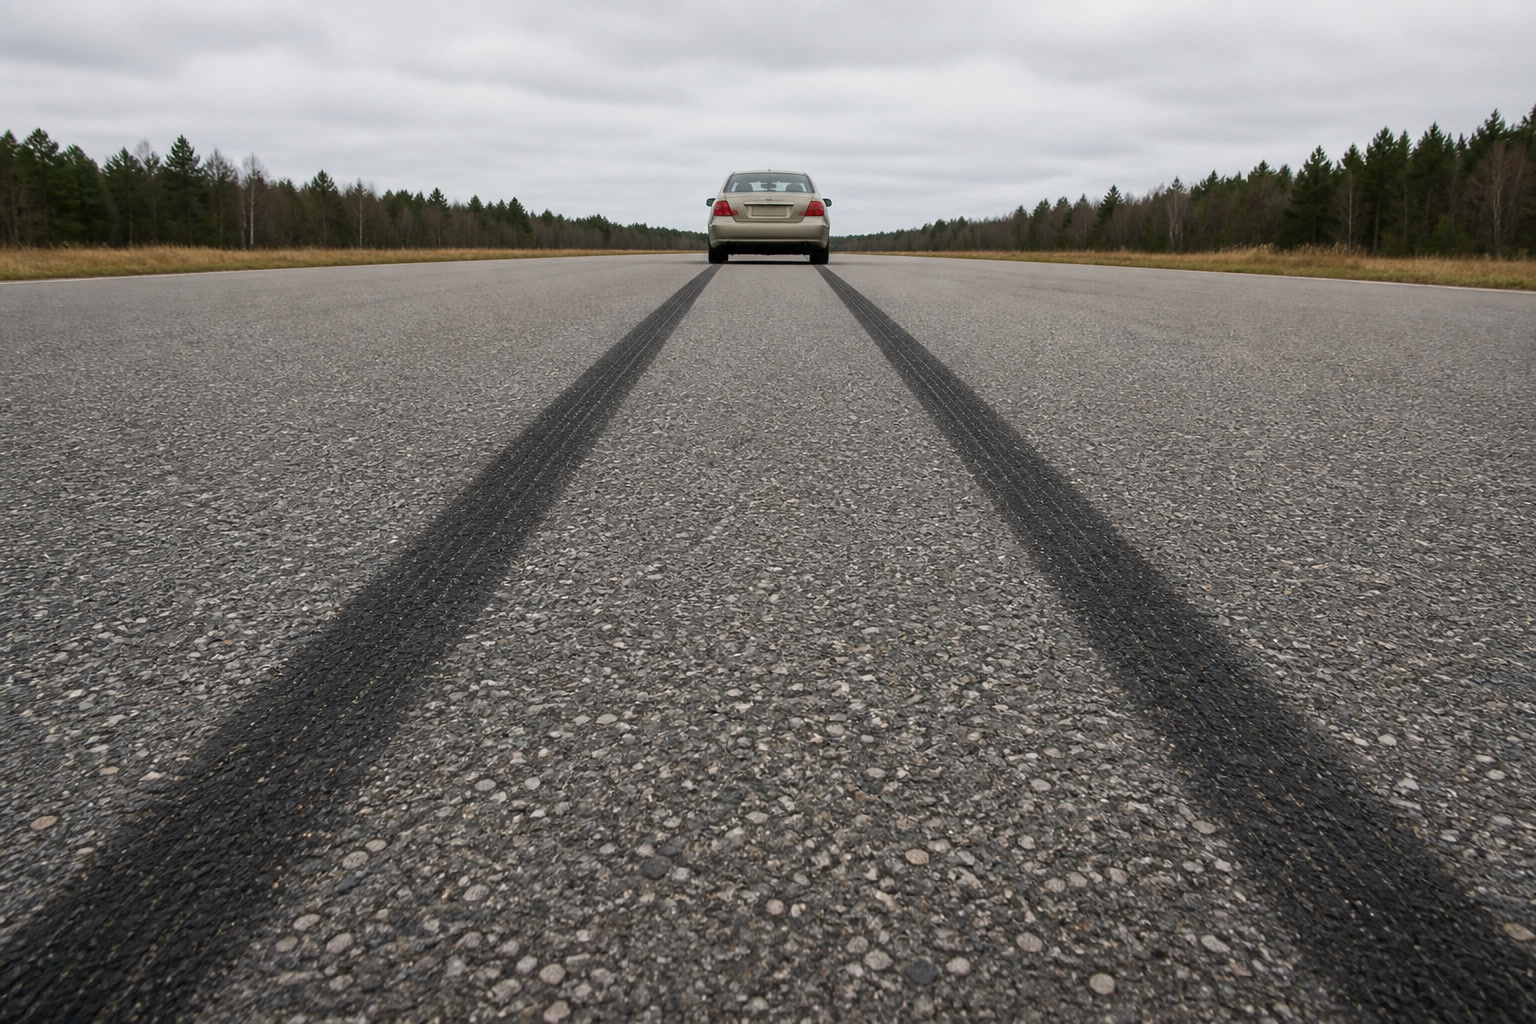
\includegraphics[width=0.55\linewidth]{images/book1/ai/g9-kinetic-skid-marks.jpg}

{\small 动能的去向：刹车与路面将其转化为热量，轮胎则在路面上留下了印记，作为凭证。}
\end{omfigure}

\section{停车距离}

\begin{proposition}[停车 = 反应 + 制动]\label{prop:g9:kinetic-energy-safety:stopping}
驾驶员发现险情后，
要经过两段路程才能停下：
\begin{enumerate}
  \item \emph{反应距离}\index{反应距离}：
        从大脑察觉险情到脚开始移动这段时间内所行驶的路程，
        速度不变时约为一秒的行驶量，因此这段距离
        与 $v$ \emph{成正比}增长；
  \item \emph{制动距离}\index{制动距离}：
        刹车使动能退场所需的路程 ---
        由于 $E_k$ 含有 $v^2$，这段距离随速度的
        \emph{平方}增长：速度加倍，
        制动距离便增至四倍。
\end{enumerate}
两者之和，即\emph{停车距离}，
正是那个追球的孩子所遭遇的数字。
\end{proposition}

\begin{example}[每位驾驶员都应掌握的表格]\label{ex:g9:kinetic-energy-safety:table}
干燥路面，驾驶员警觉（反应时间一秒，刹车性能良好）：
\begin{center}
\begin{tabular}{l|c|c|c}
速度 & 反应距离 & 制动距离 & 停车距离 \\
\hline
\qty{50}{km/h} & \qty{14}{m} & \qty{13}{m} & \qty{27}{m} \\
\qty{90}{km/h} & \qty{25}{m} & \qty{40}{m} & \qty{65}{m} \\
\qty{130}{km/h} & \qty{36}{m} & \qty{85}{m} & \qty{121}{m}
\end{tabular}
\end{center}
请仔细读两遍。城市车速下，停车距离约为一个半公交车长；
高速公路车速下，约为一条标准跑道的全长再加五分之一。
比例也印证了两条规律：反应距离随 $v$ 增长，
制动距离随 $v^2$ 增长 --- 高速行驶时，制动距离
占去了总距离的大部分。
\end{example}

\begin{method}[估算停车距离]\label{met:g9:kinetic-energy-safety:estimate}
\begin{enumerate}
  \item 将速度换算为 \unit{m/s}（把 \unit{km/h}
        数值除以 $3.6$）；
  \item 反应距离：一秒内行驶的距离 --- 即
        \unit{m/s} 的数值本身，单位为米；
  \item 制动距离：以已知参照值按平方比例换算 ---
        即从 \qty{50}{km/h} 时的 \qty{13}{m} 出发，乘以
        $(v/50)^2$；
  \item 相加，并与前方道路实际可供的
        通行距离相比较。
\end{enumerate}
路面潮湿时，制动距离会加倍；疲劳或分心的
驾驶员会使反应时间延长至接近两秒 ---
请用真实的输入值重新计算总和。
\end{method}

\begin{example}[一瞥的代价]\label{ex:g9:kinetic-energy-safety:glance}
在 \qty{90}{km/h} 时用两秒钟瞥一眼手机：汽车
行驶了 $2 \times 25 = \qty{50}{m}$ --- 约为半个足球场的长度
--- 尚未等到任何一秒的反应时间开始，就已盲目驶过。
在城市车速下，同样一瞥会盲目消耗 \qty{28}{m}：
驶过路口，驶过校门。
汽车中最危险的部件，是本节中任何公式都无法
度量的：驾驶员的注意力。
\end{example}

\begin{remark}[安全带、安全气囊与头盔]\label{rem:g9:kinetic-energy-safety:belts}
碰撞时，汽车在约一米的车身压溃中停下 --- 但
未系安全带的乘客仍以原速前行（上一章那句
平静的话，此刻残酷地应验），直到被
途中所遇之物挡住：仪表盘、挡风玻璃、路面。安全带与
安全气囊则在更长的距离和时间内让身体停下，
使其动能温和地消散，而非一次性完成；
骑车人的头盔对颅骨
内那些无法替代的东西起到同样作用，其可压碎的泡沫
为之争取了数厘米的温和制动距离。它们都不能使你的
$E_k$ 减少哪怕一焦耳 --- 它们只是让其消散变得文明。
\end{remark}

\section{练习}

\begin{exercise}[$\star$]\label{exo:g9:kinetic-energy-safety:1}
写出能量的单位及其两个参照值，并写出
动能公式以及公式中各量的单位。
\end{exercise}

\begin{exercise}[$\star$]\label{exo:g9:kinetic-energy-safety:2}
计算 $E_k$：质量为 \qty{2}{kg}、速度为 \qty{10}{m/s} 的野兔；
质量为 \qty{80}{kg}、速度为 \qty{5}{m/s} 的橄榄球运动员。
\end{exercise}

\begin{exercise}[$\star$]\label{exo:g9:kinetic-energy-safety:3}
哪种做法能使汽车的 $E_k$ 增加得更多：加上相当于
其质量一半的货物，还是把速度提高一半？请写出两种情形各自的因子。
\end{exercise}

\begin{exercise}[$\star$]\label{exo:g9:kinetic-energy-safety:4}
说出停车距离的两个组成部分，及其
增长规律：一段正比于速度，另一段正比于速度的平方。
\end{exercise}

\begin{exercise}[$\star$]\label{exo:g9:kinetic-energy-safety:5}
根据驾驶员表格，停车距离中制动距离所占的
比例在 \qty{50}{km/h} 时是多少 --- 在 \qty{130}{km/h} 时又是多少？
这一比例发生了什么变化？
\end{exercise}

\begin{exercise}[$\star$]\label{exo:g9:kinetic-energy-safety:6}
制动时，汽车的动能去了哪里？请举出你能闻到的气味
和看到的灼热之光 --- 以及那条禁止动能凭空消失的
儿时就学过的定律。
\end{exercise}

\begin{exercise}[$\star$]\label{exo:g9:kinetic-energy-safety:7}
计算速度分别为 \qty{36}{km/h}、
\qty{72}{km/h} 和 \qty{108}{km/h} 时的反应距离（取警觉的一秒）。
这些结果呈现出怎样的简单规律？
\end{exercise}

\begin{exercise}[$\star$]\label{exo:g9:kinetic-energy-safety:8}
为什么安全带不能减少你的动能 --- 它
转而使什么的消散变得文明？
\end{exercise}

\begin{exercise}[$\star\star$]\label{exo:g9:kinetic-energy-safety:9}
一辆滑板车在 \qty{30}{km/h} 时的制动距离为 \qty{8}{m}。
试估算其在 \qty{60}{km/h} 和 \qty{90}{km/h} 时的制动距离，并
说明你所依据的换算规律。
\end{exercise}

\begin{exercise}[$\star\star$]\label{exo:g9:kinetic-energy-safety:10}
各地市镇议会把学校周边路段的限速从 \qty{50}{} 降至
\qty{30}{km/h}。比较两种情况下的停车距离（参照：
在 $50$ 时制动距离为 \qty{13}{m}，反应时间取一秒）--- 并
比较两者的动能。你认为哪一种比较
在海报上更有说服力？
\end{exercise}

\begin{exercise}[$\star\star$]\label{exo:g9:kinetic-energy-safety:11}
降雨使制动距离加倍。请重新计算驾驶员表格中
潮湿路面在 $50$ 和 \qty{90}{km/h} 时的停车距离一栏 ---
你将哪一部分加倍了，哪一部分没有，为什么？
\end{exercise}

\begin{exercise}[$\star\star\star$]\label{exo:g9:kinetic-energy-safety:12}
一辆质量为 \qty{20000}{kg} 的卡车以 \qty{90}{km/h} 的速度行驶。计算
其 $E_k$（用科学记数法表示）；求出一辆质量为
\qty{1000}{kg} 的汽车获得相同动能时的速度（令两式
相等 --- 代数运算留给你今年完成）；并
总结为何山区公路上设有失控卡车避险车道，
而汽车却无此类车道。
\end{exercise}

\section{问题：安全宣传活动}

\begin{problem}[{周末问题 --- 班级设计镇上的
道路安全宣传活动；海报用公式检验；
市长的难题}]\label{pb:g9:kinetic-energy-safety:1}
镇上委托开展一项宣传活动，条件只有一个：
每张海报上的每个数字都必须经得起物理审核。
班级动手计算。（已知条件：反应时间为一秒；制动
距离在 \qty{50}{km/h} 下为 \qty{13}{m}，按平方关系换算；汽车
质量为 \qty{1000}{kg}。）

\medskip\noindent\textbf{第一部分 --- 海报一：“50 而非
60”。}
\begin{enumerate}
  \item 以 \unit{m/s} 为单位，计算两个速度（保留一位小数）。
  \item 两种速度下的反应距离各是多少？
  \item 两种速度下的制动距离各是多少（按已知条件换算）？
  \item 海报标题：“速度每增加十个单位，
        停车距离多出多少米？”请填写
        该数字。
\end{enumerate}

\medskip\noindent\textbf{第二部分 --- 海报二：“速度之
墙”。}
设计图以下落高度表示碰撞能量：速度为
$v$ 的碰撞“相当于”从某一高度下落，
即下落所获能量与之相同的那一高度。
\begin{enumerate}[resume]
  \item 计算汽车在 \qty{50}{km/h} 时的 $E_k$（数据取自
        第一部分），以及 \qty{90}{km/h} 时的动能。
  \item 美工需要高度数据：对本车而言，从 \qty{1}{m} 高处下落
        约获得 \qty{9.8}{kJ} 的能量（$m g h$ 为
        下一章的公式，此处提前借用）。两种碰撞能量
        分别对应多高的下落高度？
        （请做除法，结果取整到米。）
  \item 哪些日常建筑的高度与之相当？拟定
        海报上的文案。
  \item 市长提出异议：“没有人会直接撞墙；
        汽车会变形，安全带会拉住人。”请在承认其
        观点的同时为海报的物理内容辩护——吸能区与
        安全带改变了什么，
        又有哪些数值并未改变？
\end{enumerate}

\medskip\noindent\textbf{第三部分 --- 海报三：“一
秒”。}
\begin{enumerate}[resume]
  \item 以 \qty{90}{km/h} 行驶时，
        分心一秒在开始制动前要耗去多少米？再看
        两秒钟的手机一瞥呢？
  \item 疲劳驾驶版本：反应时间延长到两
        秒。重新计算
        \qty{90}{km/h} 下的完整停车距离，并与清醒驾驶员的
        \qty{65}{m} 作比较。
  \item 一位持怀疑态度的议员说：“与那些很大的制动数字相比，
        一秒钟应该无足轻重吧。”他在哪种速度下错得最离谱——
        低速还是高速？（比较两项距离的增长规律。）
        的两个分量的增长规律。）
  \item 定稿宣传活动：三张海报的底部各写一行字，
        每张一行，各配一条公式，
        用通俗的语言表述。
\end{enumerate}
\end{problem}
